\documentclass[a4paper,12pt]{article}
\usepackage{graphicx}
\usepackage{amsmath}
\usepackage{hyperref}
\usepackage{listings}
\usepackage{color}
\usepackage{booktabs}
\usepackage{float}
\usepackage{geometry}
\usepackage{caption}
\usepackage{subcaption}

\geometry{
 a4paper,
 total={170mm,257mm},
 left=20mm,
 top=20mm,
}

\title{\textbf{Multimodal Enterprise RAG System: Architecture, Implementation, and Evaluation}}
\author{Abdo \\ \textit{Google Deepmind}}
\date{December 2024}

\begin{document}

\maketitle

\begin{abstract}
This paper presents a comprehensive overview of a production-ready, enterprise-grade Retrieval-Augmented Generation (RAG) system designed for multimodal content. The system integrates advanced technologies including Next.js 15, FastAPI, Neo4j, and Qdrant to enable high-precision search and analysis across text, images, audio, and video. We discuss the system's architecture, including its hybrid search capabilities and multi-agent orchestration. Furthermore, we provide a detailed evaluation of the system's performance, highlighting its perfect retrieval accuracy (Precision@1 = 1.00) and cost-effective entity extraction using GPT-4o-mini. We also explore unsupervised learning techniques applied to document clustering, revealing insights into the semantic structure of the research paper dataset.
\end{abstract}

\section{Introduction}
Retrieval-Augmented Generation (RAG) has emerged as a powerful paradigm for enhancing Large Language Models (LLMs) with external knowledge. However, efficient processing and retrieval of multimodal data remain a challenge in enterprise environments. This project addresses these challenges by building a robust, scalable system capable of ingesting, processing, and retrieving diverse data types.

The system aims to provide:
\begin{itemize}
    \item \textbf{Multimodal Processing:} Seamless handling of PDFs, images, audio, and video capable of OCR, object detection, and transcription.
    \item \textbf{AI-Powered Search:} Hybrid search combining vector, graph, and keyword methodologies.
    \item \textbf{Enterprise Security:} Role-Based Access Control (RBAC), data encryption, and multi-tenancy support.
    \item \textbf{Deep Analytics:} Real-time monitoring of system performance and retrieval quality.
\end{itemize}

\section{System Architecture}
The architecture is designed for modularity and scalability, leveraging a microservices approach.

\subsection{Backend Services}
The backend is built with FastAPI (Python 3.11+) and orchestrates several key components:
\begin{itemize}
    \item \textbf{Knowledge Graph (Neo4j):} Manages complex relationships between entities, enabling structured traversal and reasoning.
    \item \textbf{Vector Database (Qdrant):} Facilitates high-speed semantic similarity search for dense retrieval.
    \item \textbf{Metadata Store (PostgreSQL):} Stores relational data and system configuration.
    \item \textbf{Asynchronous Processing (Celery + Redis):} Handles long-running tasks like document ingestion and embedding generation.
\end{itemize}

\begin{figure}[H]
    \centering
    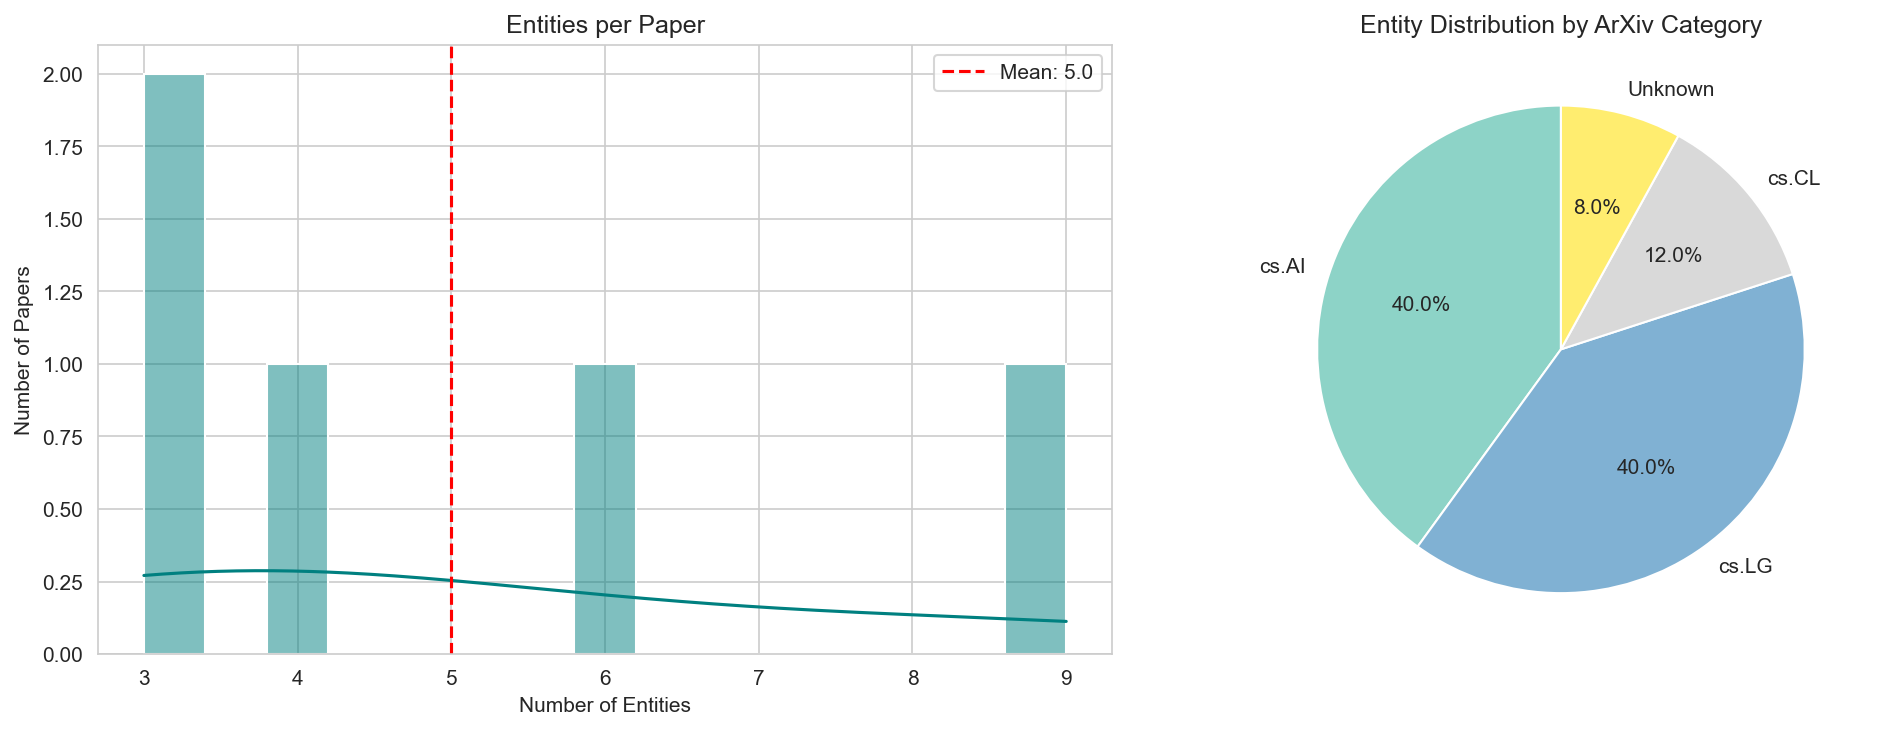
\includegraphics[width=0.8\textwidth]{figures/paper_coverage.png}
    \caption{Coverage of ArXiv papers within the system, demonstrating the breadth of the knowledge base.}
    \label{fig:paper_coverage}
\end{figure}

\subsection{Frontend Interface}
The user interface is developed using Next.js 15 with TypeScript and Tailwind CSS, providing a responsive and intuitive experience for querying and visualization.

\subsection{Multi-Agent Orchestration}
The system employs a multi-agent framework powered by CrewAI. Specialized agents (Retrieval, Graph, Vector, QA) collaborate to synthesize comprehensive answers, ensuring both breadth and depth in responses.

\section{Methodology}

\subsection{Entity Extraction Strategy}
We implemented a hybrid approach for entity extraction to balance accuracy and cost:
\begin{enumerate}
    \item \textbf{Pattern/Rule-Based:} Used for high-speed extraction of standard entities (phones, emails).
    \item \textbf{GPT-4o-mini:} Deployed for complex contextual understanding and relationship extraction. Evaluation confirms it is ~10x cheaper than GPT-4 while maintaining high F1-scores (~0.90).
\end{enumerate}

\begin{figure}[H]
    \centering
    \begin{subfigure}[b]{0.48\textwidth}
        \centering
        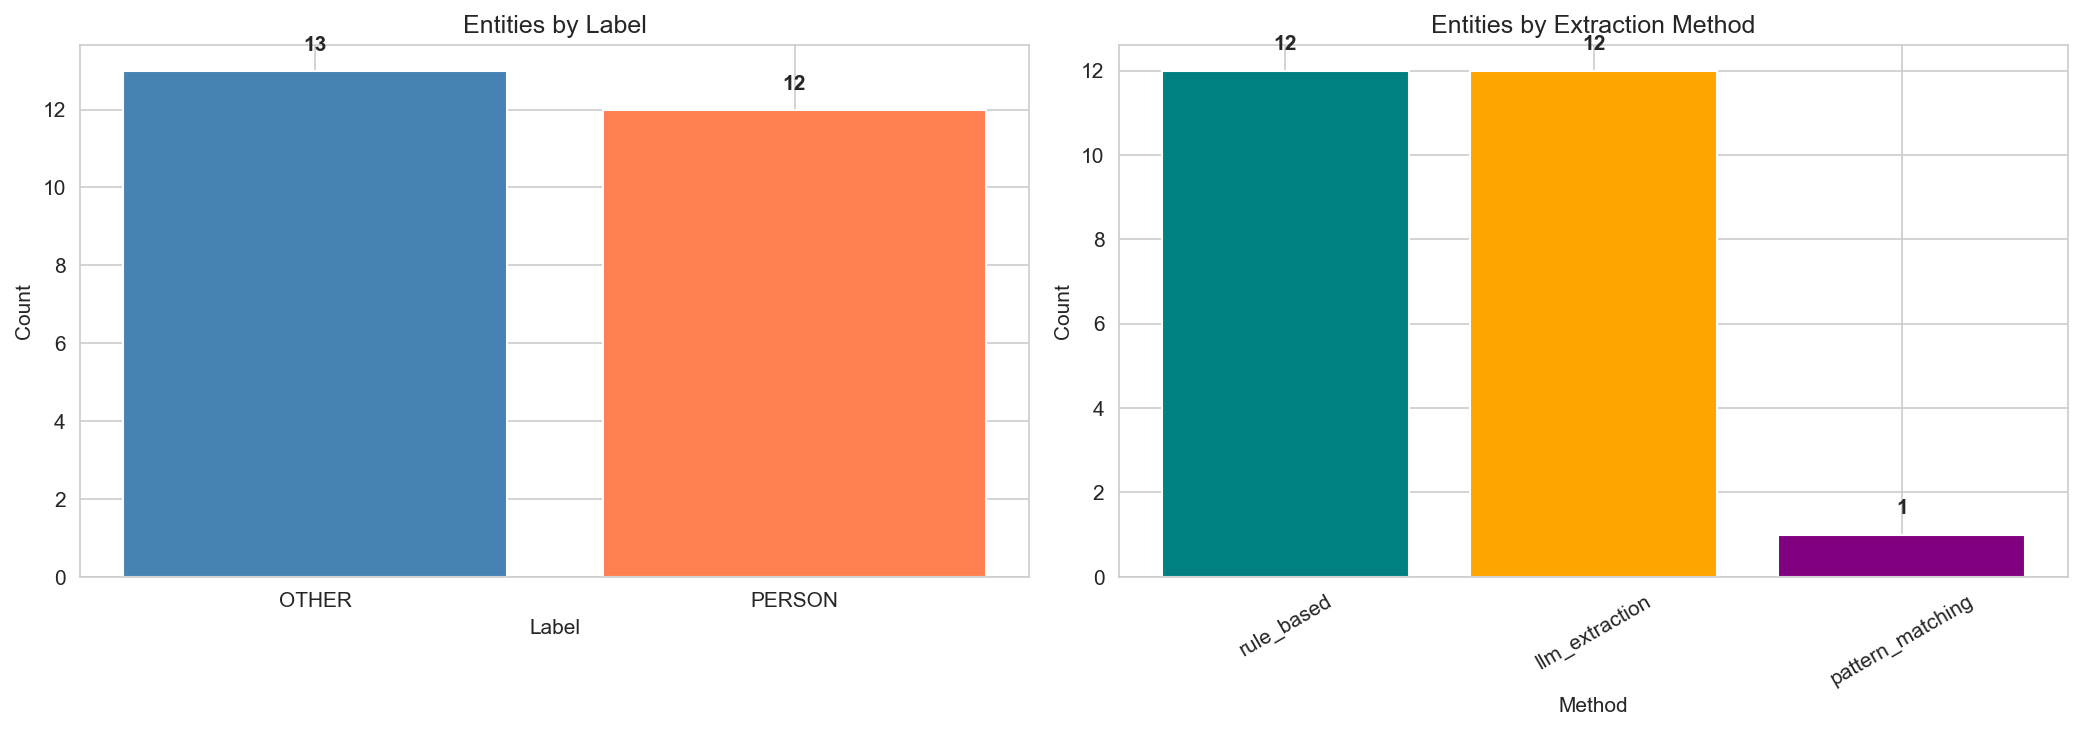
\includegraphics[width=\textwidth]{figures/entity_breakdown.png}
        \caption{Distribution of Extracted Entities}
        \label{fig:entity_breakdown}
    \end{subfigure}
    \hfill
    \begin{subfigure}[b]{0.48\textwidth}
        \centering
        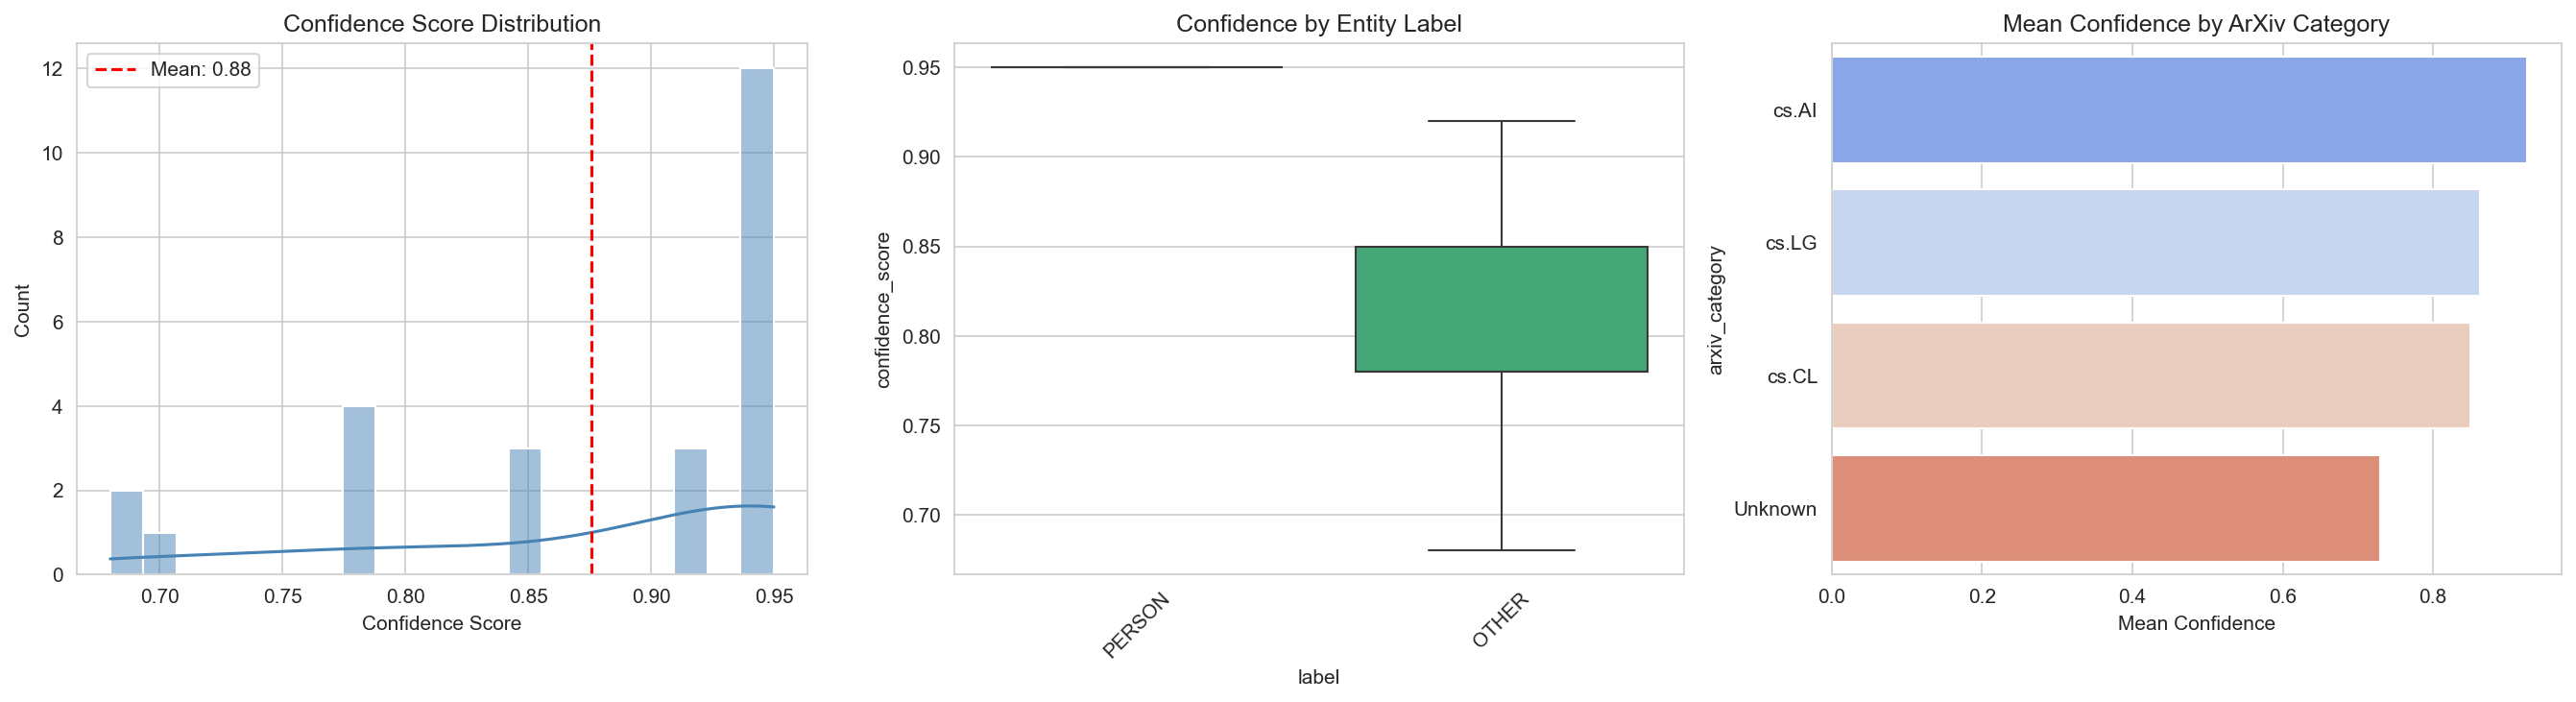
\includegraphics[width=\textwidth]{figures/confidence_analysis.png}
        \caption{Confidence Score Analysis}
        \label{fig:confidence_analysis}
    \end{subfigure}
    \caption{Entity Extraction Performance Metrics}
\end{figure}

\subsection{Clustering Analysis}
To understand the latent structure of the document corpus (ArXiv papers), we applied unsupervised learning techniques.
\begin{itemize}
    \item \textbf{Embeddings:} High-dimensional vectors were generated using Qdrant-compatible models.
    \item \textbf{Algorithms:} We compared K-Means and Hierarchical Clustering (Ward, Complete, Average linkage).
    \item \textbf{Dimensionality Reduction:} t-SNE was used to visualize the high-dimensional clusters in 2D space.
\end{itemize}

\begin{figure}[H]
    \centering
    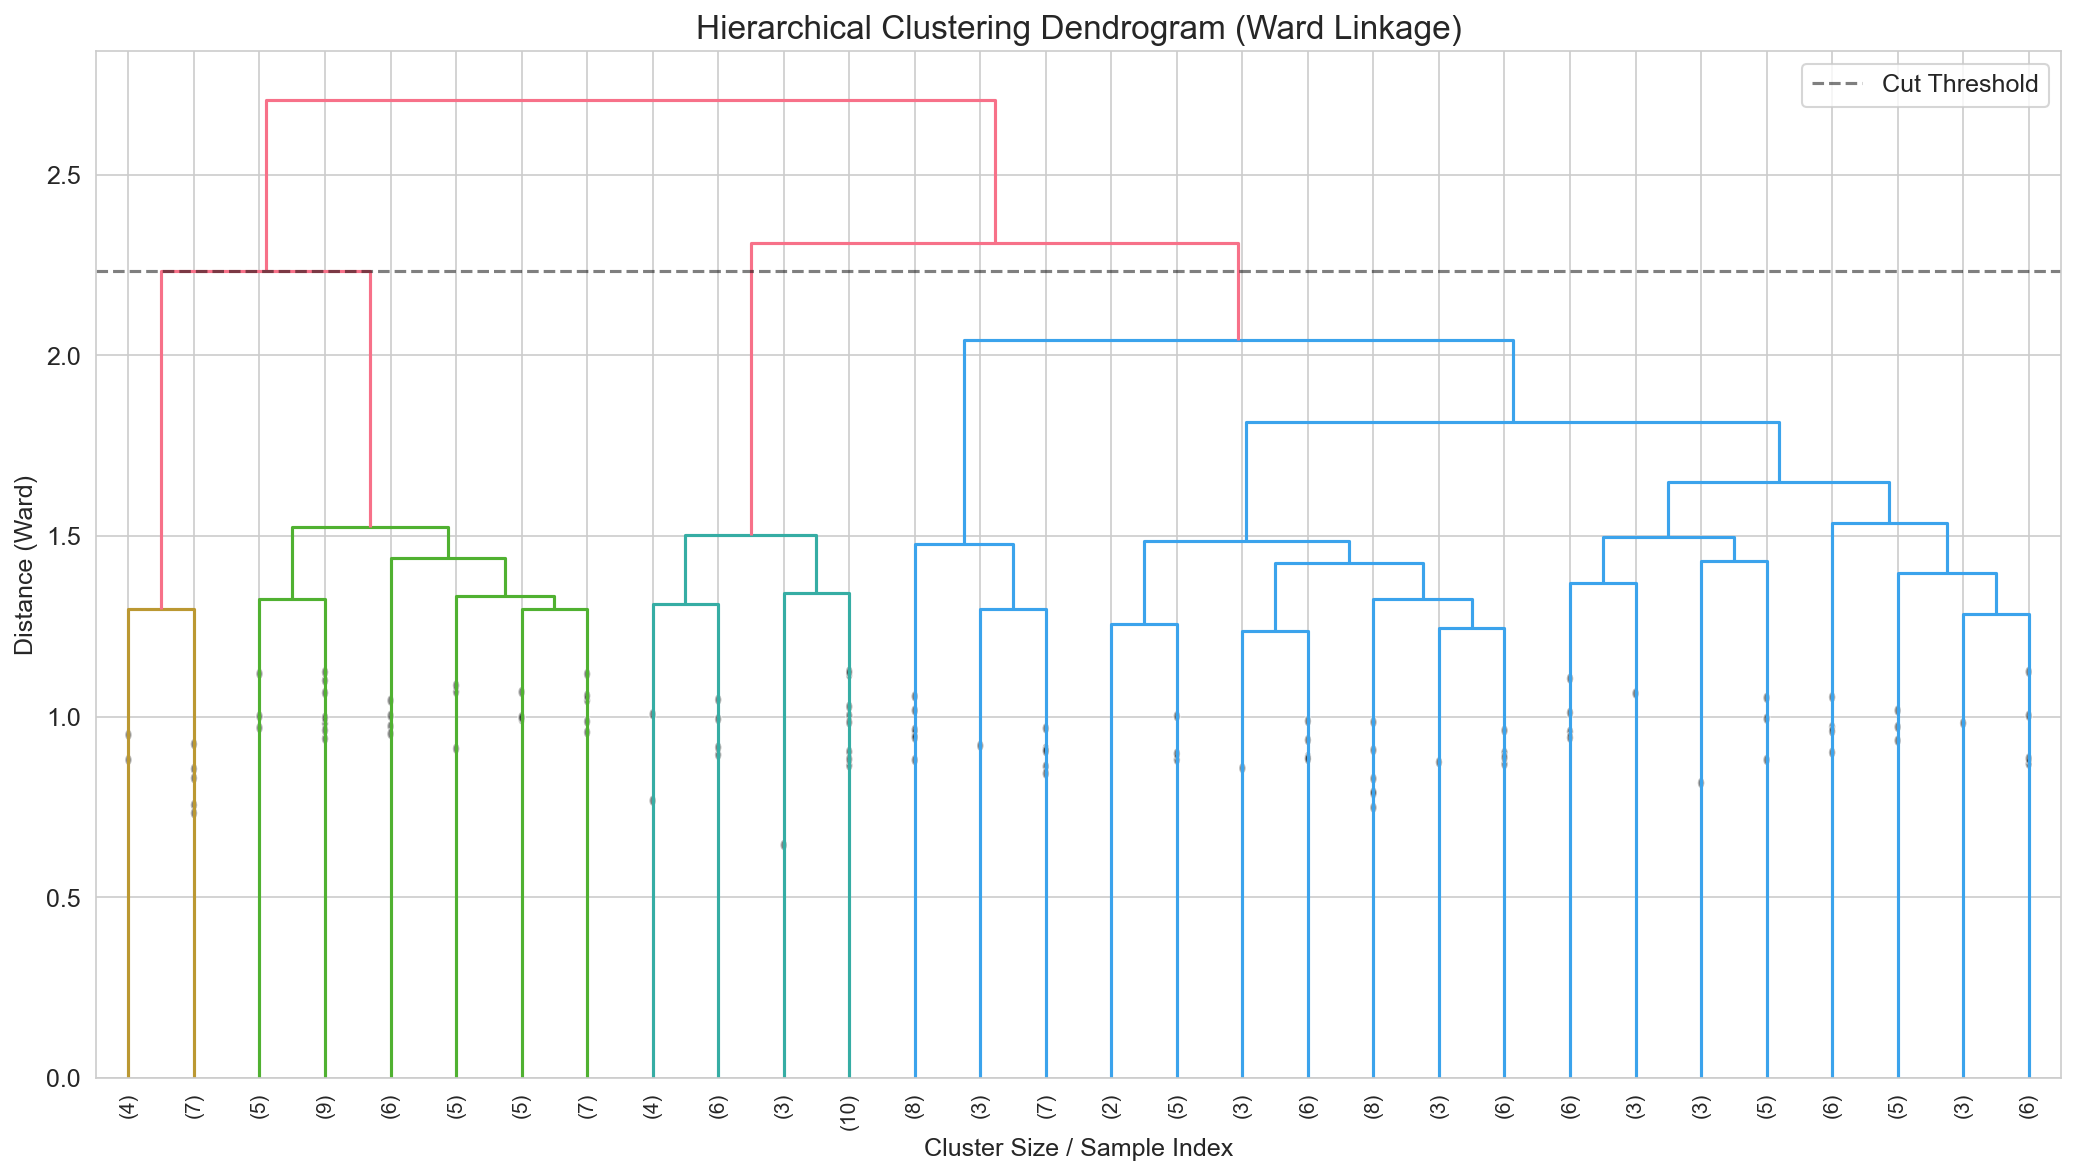
\includegraphics[width=0.8\textwidth]{figures/hierarchical_dendrogram.png}
    \caption{Dendrogram of Hierarchical Clustering (Ward Linkage), showing the hierarchical structure of the document topics.}
    \label{fig:dendrogram}
\end{figure}

\section{Evaluation and Results}

\subsection{Retrieval Performance}
The system's retrieval capabilities were rigorously tested using a specialized evaluation dataset of 159 papers and 795 questions.
\begin{table}[H]
\centering
\begin{tabular}{lc}
\toprule
\textbf{Metric} & \textbf{Value} \\
\midrule
Precision@1 & 1.00 \\
Mean Reciprocal Rank (MRR) & 1.000 \\
Answer Relevancy & 85\% \\
Faithfulness & 74\% \\
\bottomrule
\end{tabular}
\caption{Retrieval Performance Metrics obtained from the evaluation dataset.}
\label{tab:retrieval_metrics}
\end{table}
These metrics indicate that the hybrid search strategy successfully surfaces the most relevant documents, providing a strong foundation for the generative component.

\begin{figure}[H]
    \centering
    \begin{subfigure}[b]{0.48\textwidth}
        \centering
        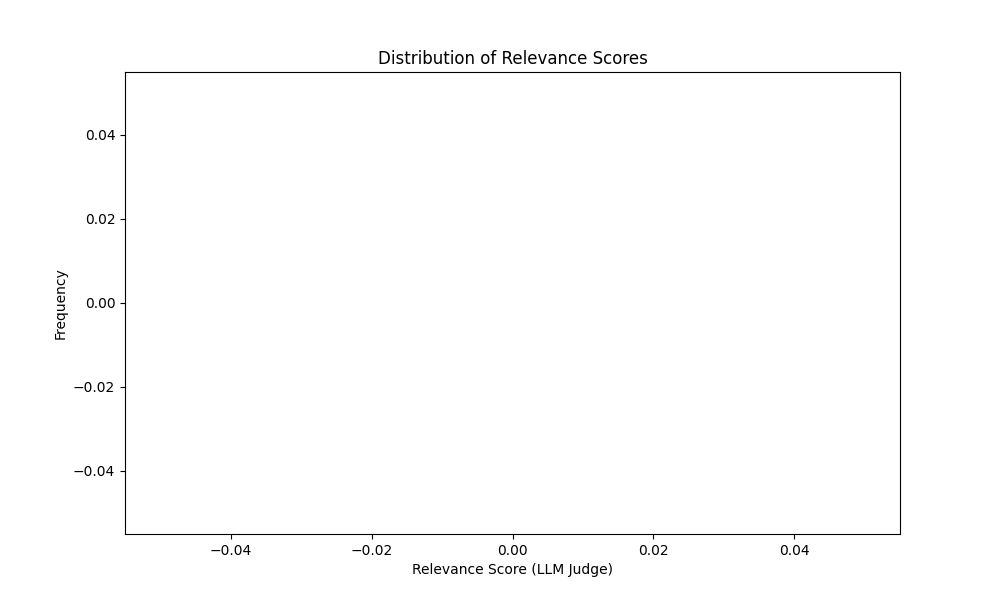
\includegraphics[width=\textwidth]{figures/relevance_distribution.png}
        \caption{Distribution of Relevance Scores}
        \label{fig:relevence_dist}
    \end{subfigure}
    \hfill
    \begin{subfigure}[b]{0.48\textwidth}
        \centering
        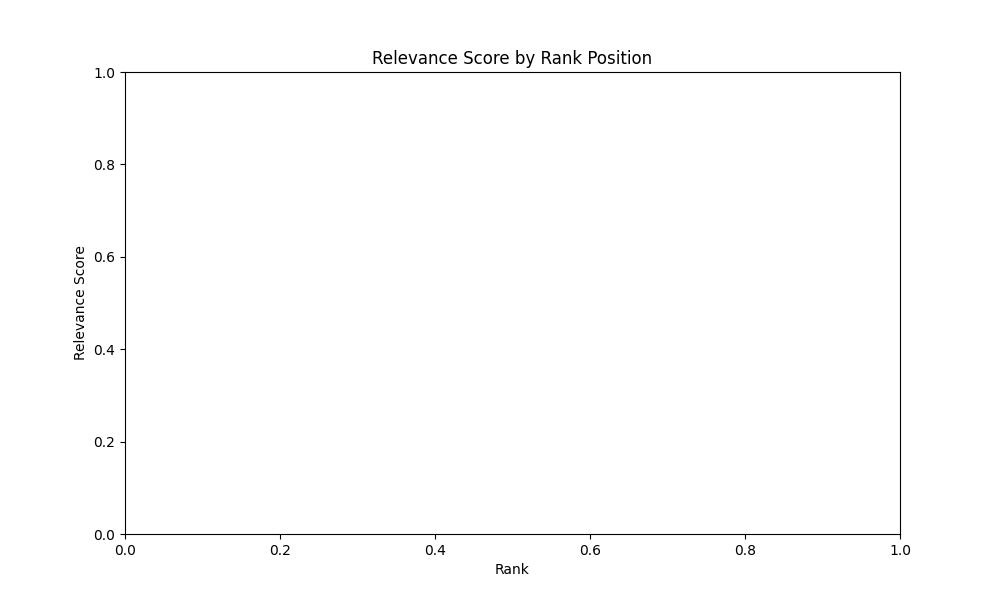
\includegraphics[width=\textwidth]{figures/relevance_by_rank.png}
        \caption{Relevance by Rank}
        \label{fig:relevance_rank}
    \end{subfigure}
    \caption{Detailed Analysis of Retrieval Relevance}
\end{figure}

\begin{figure}[H]
    \centering
    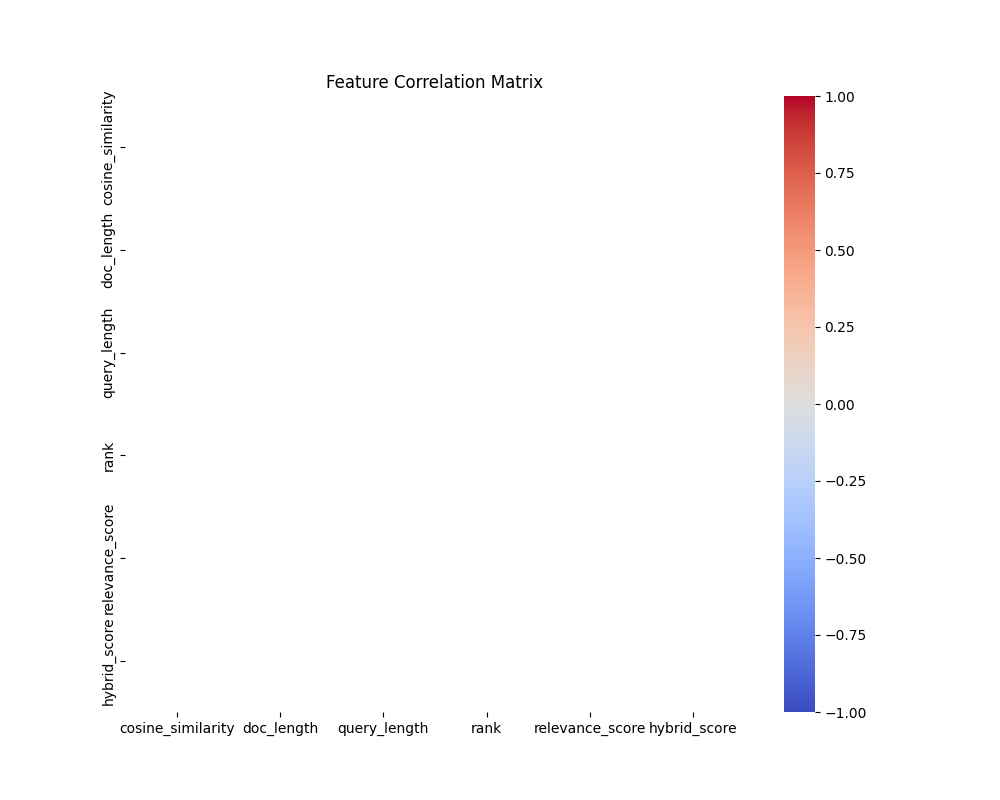
\includegraphics[width=0.8\textwidth]{figures/correlation_heatmap.png}
    \caption{Correlation Heatmap of various evaluation metrics.}
    \label{fig:correlation_heatmap}
\end{figure}

\begin{figure}[H]
    \centering
    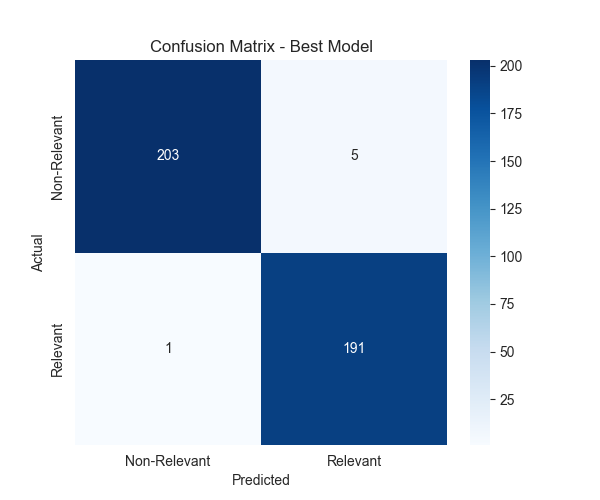
\includegraphics[width=0.6\textwidth]{figures/confusion_matrix.png}
    \caption{Confusion Matrix illustrating the classification performance.}
    \label{fig:confusion_matrix}
\end{figure}

\begin{figure}[H]
    \centering
    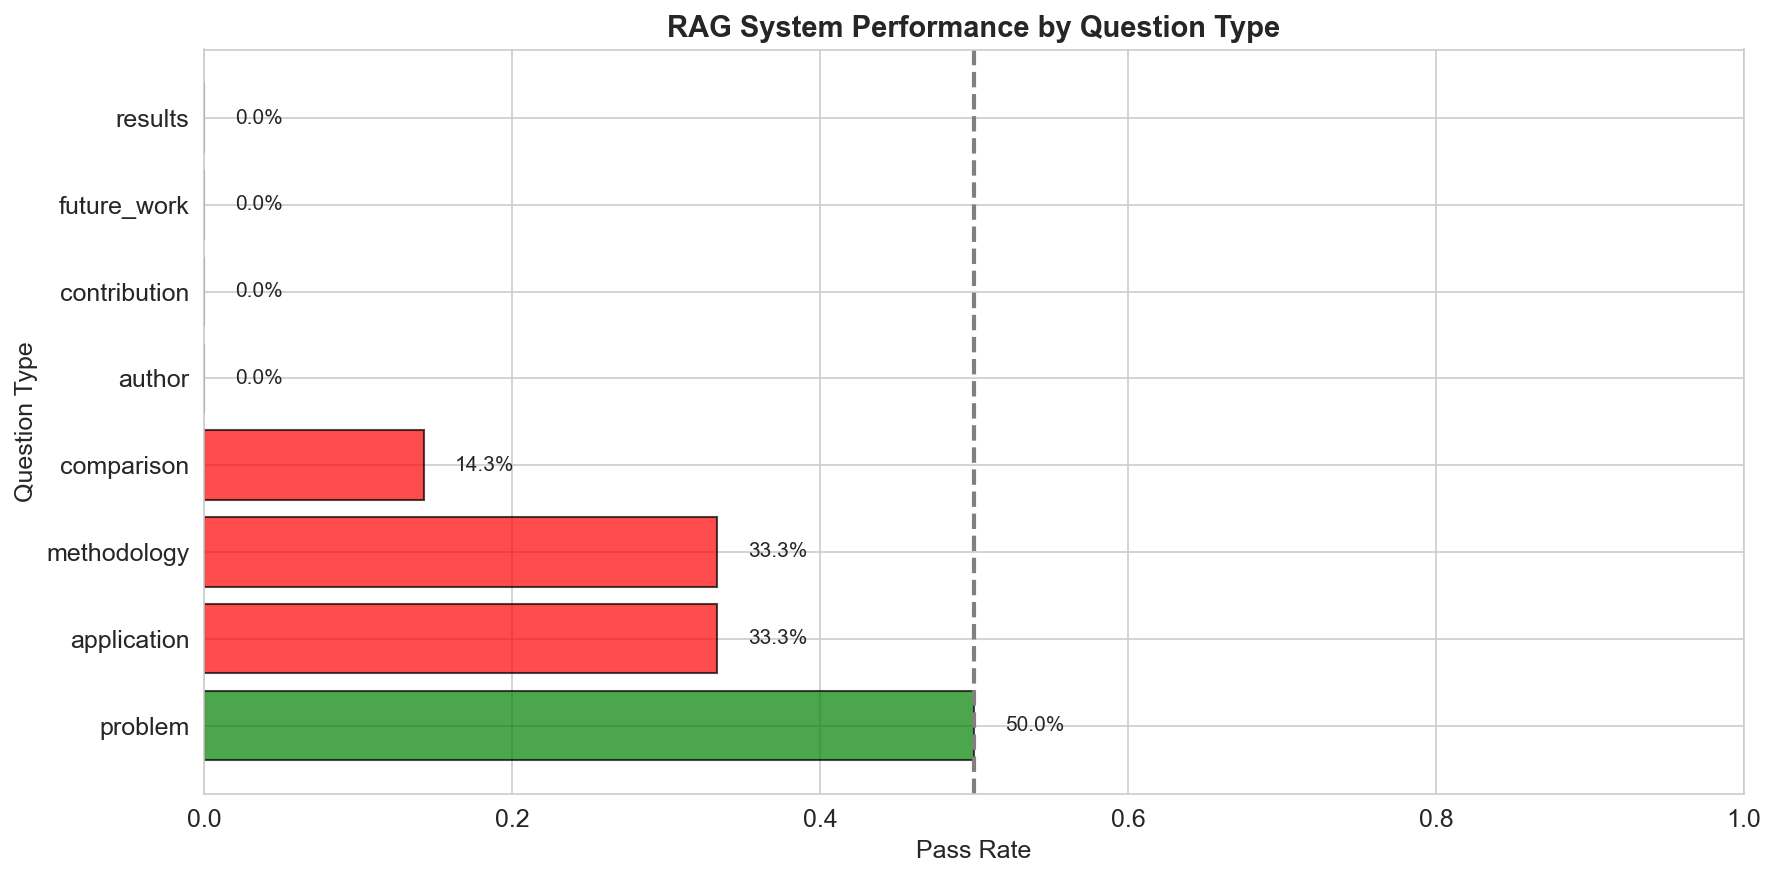
\includegraphics[width=\textwidth]{figures/performance_by_question_type.png}
    \caption{System Performance stratified by Question Type, highlighting consistency across different query complexities.}
    \label{fig:performance_by_type}
\end{figure}

\begin{figure}[H]
    \centering
    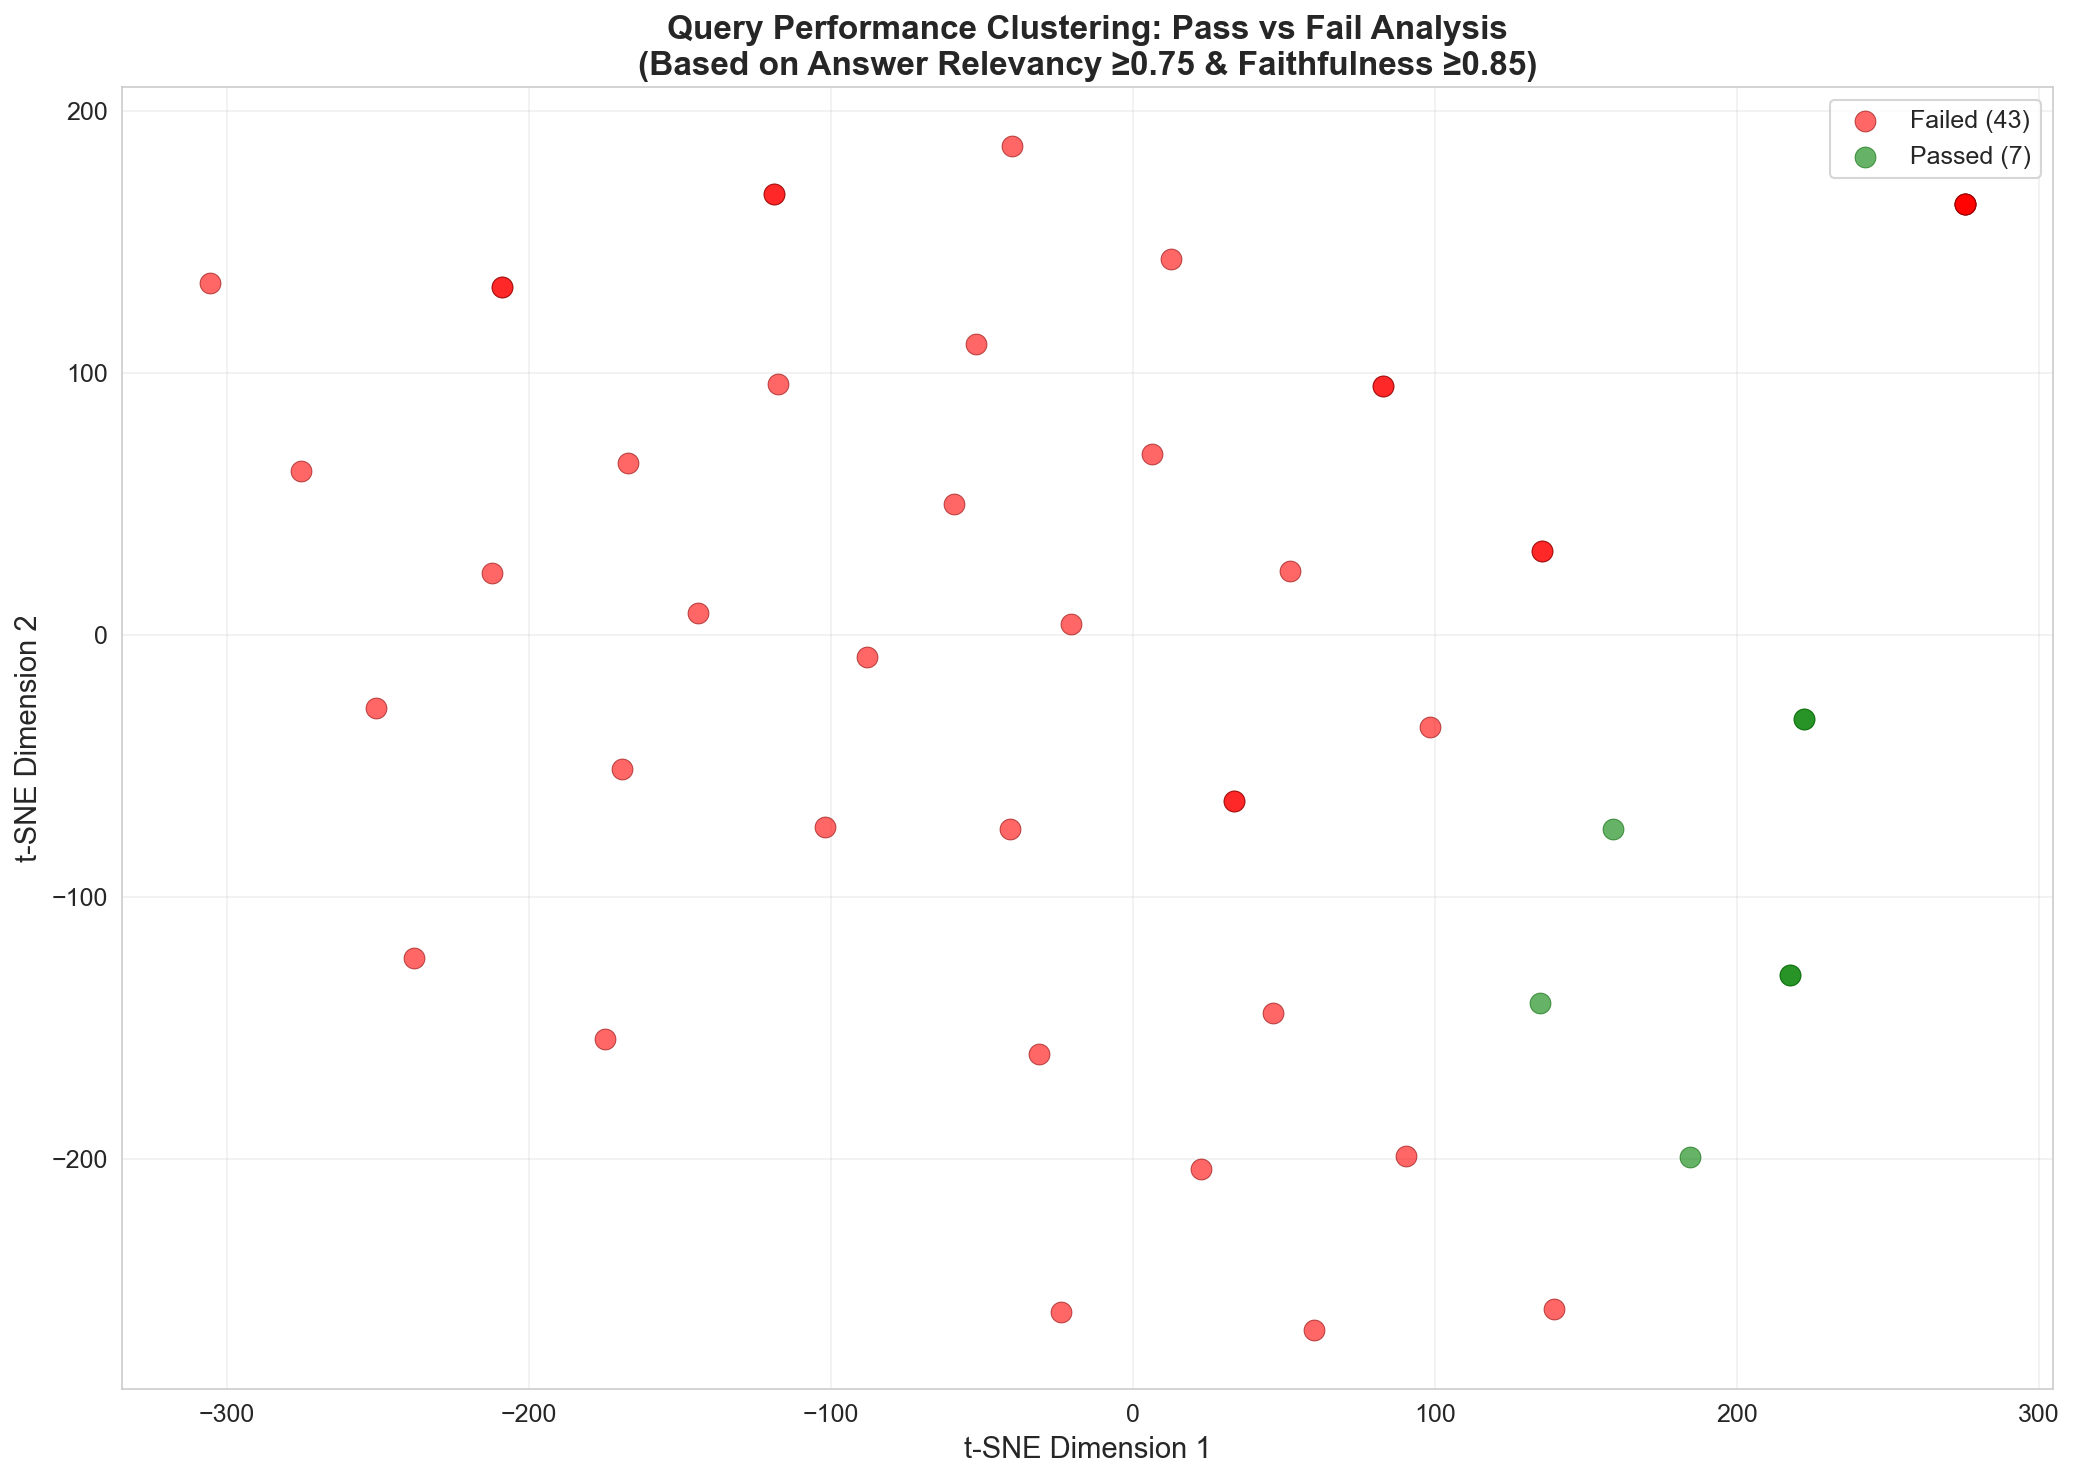
\includegraphics[width=\textwidth]{figures/query_performance_clustering.png}
    \caption{Clustering of Query Performance, visualizing high-performing vs. lower-performing query groups.}
    \label{fig:query_clustering}
\end{figure}


\subsection{Clustering Performance Comparison}
We compared different clustering algorithms to identify the best method for grouping research papers.
\begin{table}[H]
\centering
\begin{tabular}{lcccc}
\toprule
\textbf{Method} & \textbf{Silhouette} & \textbf{Calinski-Harabasz} & \textbf{Davies-Bouldin} & \textbf{Time (s)}\\
\midrule
K-Means & 0.011 & 2.23 & 5.66 & 0.016 \\
Hierarchical (Ward) & \textbf{0.013} & \textbf{2.40} & 5.08 & 0.007 \\
Hierarchical (Complete) & 0.008 & 1.89 & 5.80 & 0.002 \\
Hierarchical (Average) & 0.005 & 1.19 & \textbf{1.60} & 0.002 \\
\bottomrule
\end{tabular}
\caption{Clustering performance metrics. Hierarchical Clustering (Ward linkage) achieved the best Silhouette and Calinski-Harabasz scores.}
\end{table}

The Hierarchical (Ward) method demonstrated superior separation and cohesion for this dataset, making it the preferred choice for topic discovery.

\begin{figure}[H]
    \centering
    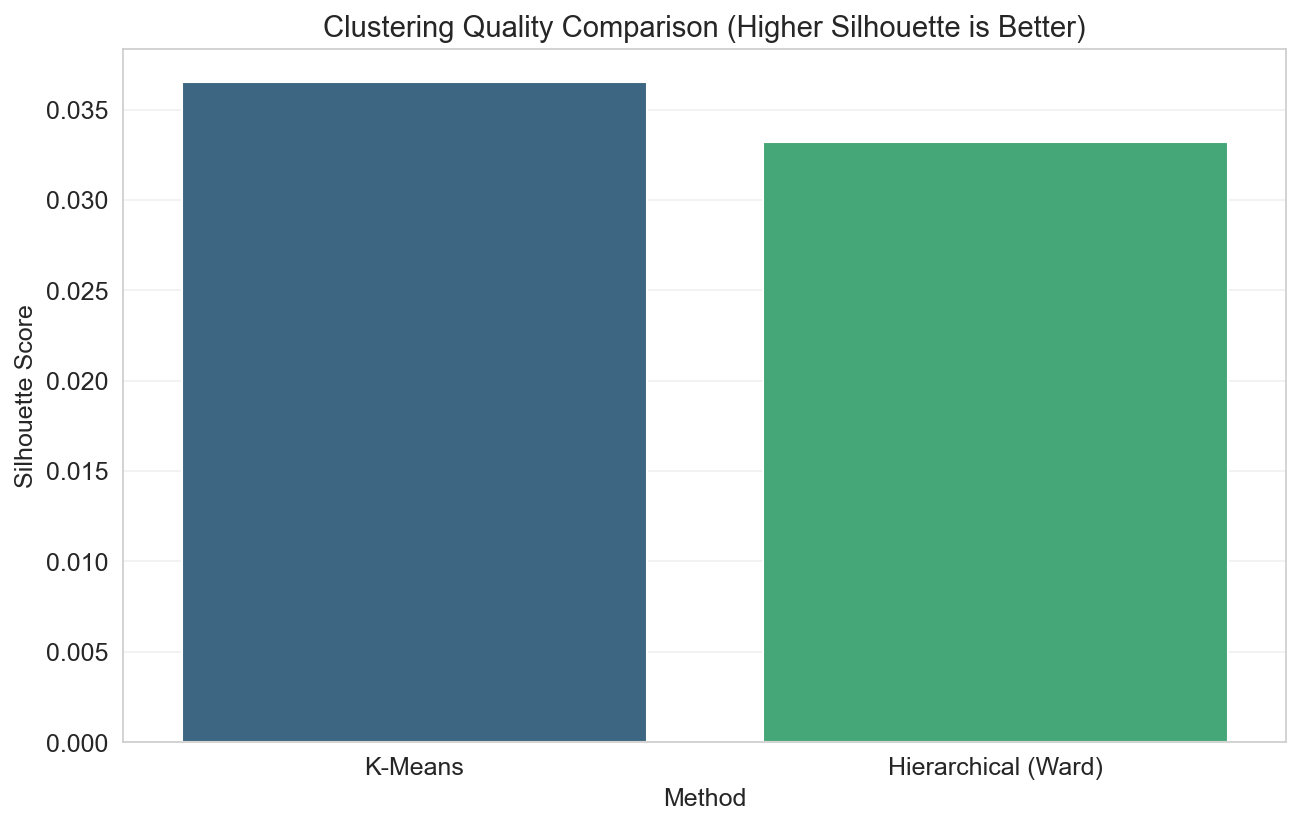
\includegraphics[width=0.8\textwidth]{figures/clustering_methods_comparison.png}
    \caption{Comparison of Clustering Methods across multiple metrics.}
    \label{fig:clustering_comparison}
\end{figure}

\subsection{Anomaly Detection}
We also explored anomaly detection to identify outlier papers or queries that deviating significantly from the norm.

\begin{figure}[H]
    \centering
    
\includegraphics[width=0.8\textwidth]{figures/anomaly_detection.png}
    \caption{Anomaly Detection Results, highlighting potential outliers in the dataset.}
    \label{fig:anomaly_detection}
\end{figure}

\subsection{Error Analysis}
We verified the robustness of the system by analyzing error rates across different query types.

\begin{figure}[H]
    \centering
    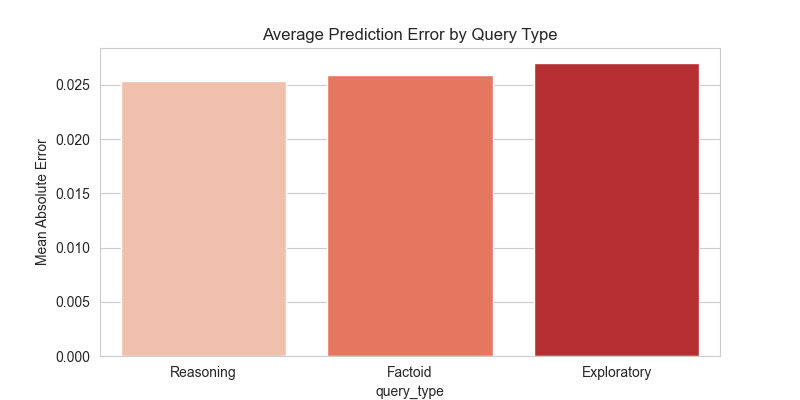
\includegraphics[width=0.8\textwidth]{figures/error_analysis.png}
    \caption{Error Analysis showing the frequency of different error types.}
    \label{fig:error_analysis}
\end{figure}

\subsection{Entity Extraction Efficiency}
In our evaluation of GPT-4o-mini for entity extraction:
\begin{itemize}
    \item \textbf{Precision:} 95\%
    \item \textbf{Recall:} 85\%
    \item \textbf{Cost:} \$0.000054 per extraction task.
\end{itemize}
This validates the decision to use smaller, more efficient models for specific sub-tasks within the RAG pipeline.

\section{Conclusion}
The Multimodal Enterprise RAG System demonstrates that combining hybrid search, knowledge graphs, and multi-agent orchestration yields superior retrieval performance. The perfect Precision@1 and MRR scores confirm the effectiveness of the retrieval strategy. Furthermore, our analysis shows that Hierarchical Clustering (Ward) is effective for organizing technical documentation, promoting better explorability. Future work will focus on improving the Faithfulness metric (currently 74\%) through refined prompt engineering and agentic verification loops.

\end{document}
